%----------------------------------------------------------------------------------------
%	PACKAGES AND DOCUMENT CONFIGURATIONS
%----------------------------------------------------------------------------------------
\documentclass[11pt]{article}
\usepackage{amsmath} % Required for some math elements
\usepackage{hyperref} 
\usepackage{xcolor}
\usepackage{lipsum} 
\usepackage{cite}
\usepackage{graphicx} % Required for the inclusion of images
\usepackage{algorithmic}
\usepackage{array}
\usepackage{bookmark}
\usepackage{listings}
\usepackage{amssymb}
\usepackage{enumitem}
\usepackage[margin=16mm]{geometry}
\usepackage[caption=false, font=footnotesize]{subfig}
\usepackage{fancyhdr}
\renewcommand{\headrulewidth}{0.4pt}
\renewcommand{\footrulewidth}{0.4pt}

\usepackage[active,tightpage]{preview}
\renewcommand{\PreviewBorder}{1in}
\newcommand{\Newpage}{\end{preview}\begin{preview}}

\newlist{steps}{enumerate}{1}
\setlist[steps, 1]{label = Step \arabic*:}

\hypersetup{ %color attributes of citation, link, etc.
    colorlinks=true,
    linkcolor=blue,
    filecolor=gray,      
    urlcolor=blue,
    citecolor=blue,
}

\newcommand{\matlab}{\textsc{Matlab }} %very important and totally necessary addition

\newcommand\Item[1][]{%
  \ifx\relax#1\relax  \item \else \item[#1] \fi
  \abovedisplayskip=0pt\abovedisplayshortskip=0pt~\vspace*{-\baselineskip}}
%----------------------------------------------------------------------------------------
%	DOCUMENT INFORMATION
%----------------------------------------------------------------------------------------

\title{ECEN 415 \\ Assignment 1 Submission}
\author{Daniel Eisen : 300447549}
\date{\today}

\begin{document}
\begin{preview}
\maketitle

%----------------------------------------------------------------------------------------
%	DOCUMENT CONTENT
%----------------------------------------------------------------------------------------
\section*{Section A - Formative Questions}
\begin{enumerate}
    \item 
    \begin{enumerate}
        \item 
        $$G_1(s) = \frac{20(s^2 + s + 0.5)}{s(s+1)(s+10)}$$
        \begin{center}
            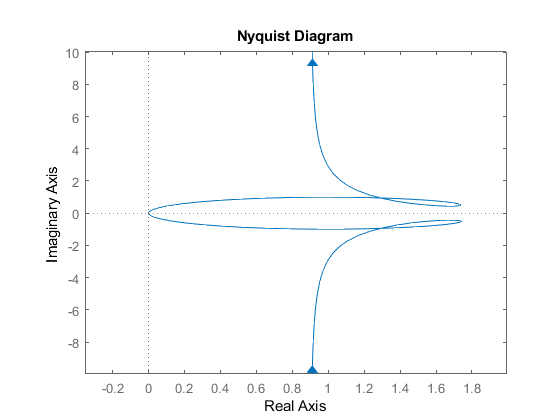
\includegraphics[width=0.33\textwidth]{fig/1a.png}
        \end{center}
        The system in its current state is stable as there are no enclosures of the critical point, and no open open-loop poles in the right half side of the s-place. No level of gain from $0 \rightarrow \infty$ result in an enclosure, and thus the system cannot be made unstable with this method.  
        \item 
        $$G_2(s) = \frac{20(s^2 + s + 0.5)}{s(s-1)(s+10)}$$
        \begin{center}
            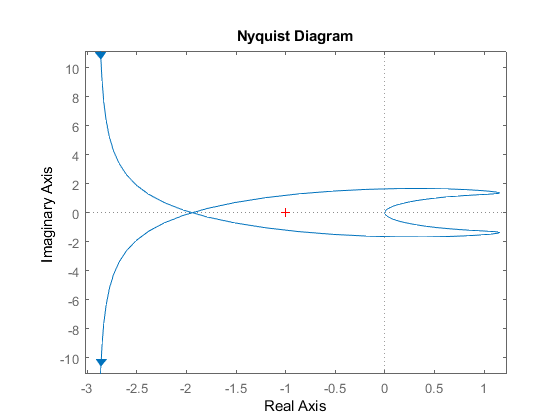
\includegraphics[width=0.33\textwidth]{fig/1b.png}
        \end{center}
        The system in its current state is stable as there is one open-loop pole in the right half side of the s-place and one anti-clockwise encirclement of the critical point. However with reduced gain, there will be no enclosure of the critical point and the system can be driven unstable.
        \item 
        $$G_3(s) = \frac{s^2 + 3}{(s+1)^2}$$
        \begin{center}
            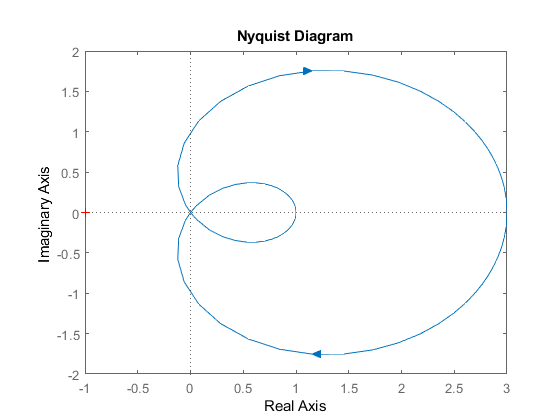
\includegraphics[width=0.33\textwidth]{fig/1c.png}
        \end{center}
        The system in its current state is stable as there are no enclosures of the critical point, and no open open-loop poles in the right half side of the s-place.  No level of gain from $0 \rightarrow \infty$ result in an enclosure, and thus the system cannot be made unstable with this method.
        \item 
        $$G_4(s) = \frac{3(s+1)}{s(s-10)}$$
        \begin{center}
            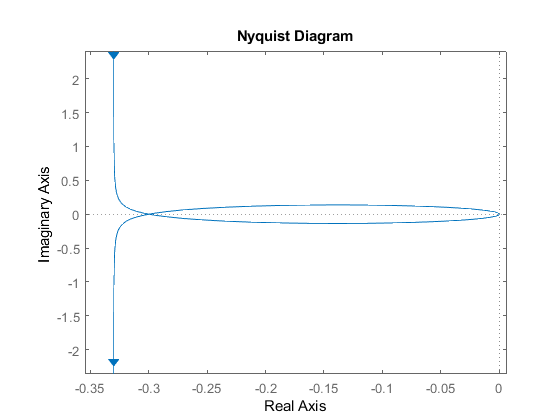
\includegraphics[width=0.33\textwidth]{fig/1d.png}
        \end{center}
        The system is currently unstable, as there is one open-loop pole in the right half side of the s-place and no anti-clockwise encirclements of the critical point. By increasing the gain we can make and anti-clockwise encirclement of the critical point and result in a stable system.
    \end{enumerate}
    \item
    $$G = e^{-0.2s}\frac{4}{s+2}$$
    \begin{enumerate}
        \item 
        \begin{center}
            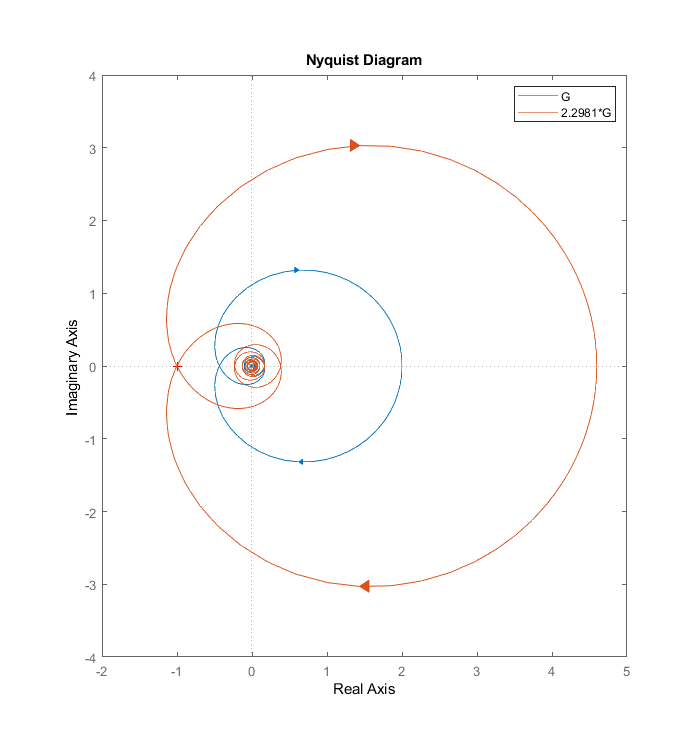
\includegraphics[width=0.33\textwidth]{fig/2a.png}
        \end{center}
        \item 
        \begin{center}
            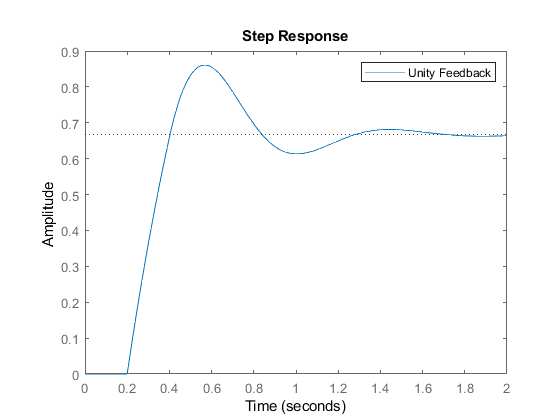
\includegraphics[width=0.33\textwidth]{fig/2bs.png}
            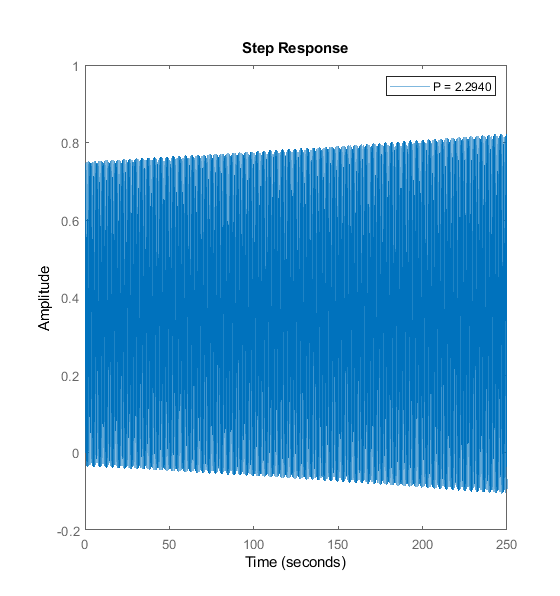
\includegraphics[width=0.33\textwidth]{fig/2bu.png}
        \end{center}
        \item 
        \begin{center}
            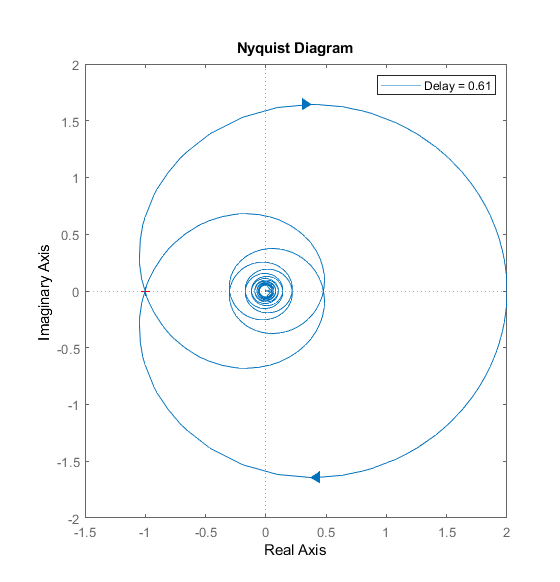
\includegraphics[width=0.33\textwidth]{fig/2c.png}
        \end{center}
    \end{enumerate} 
    \item 
    \begin{center}
        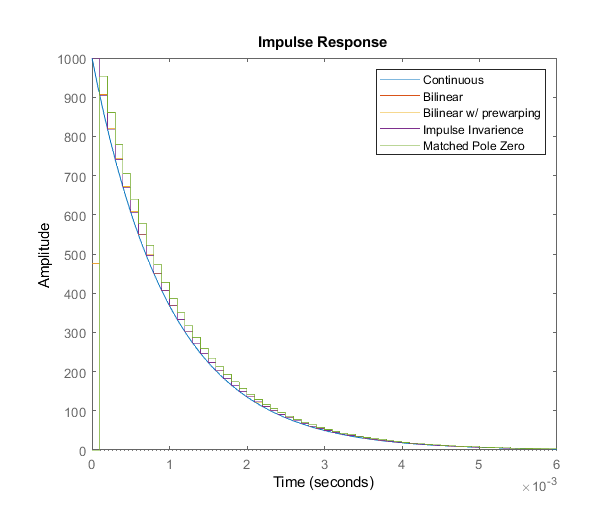
\includegraphics[height=0.3\textwidth]{fig/3_imp.png}
        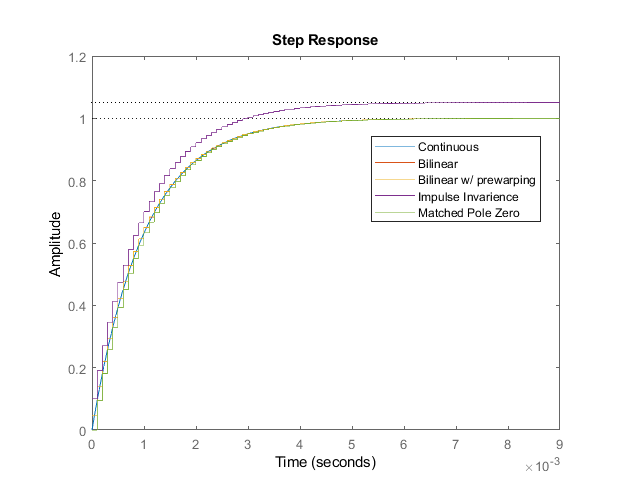
\includegraphics[height=0.3\textwidth]{fig/3_stp.png}
        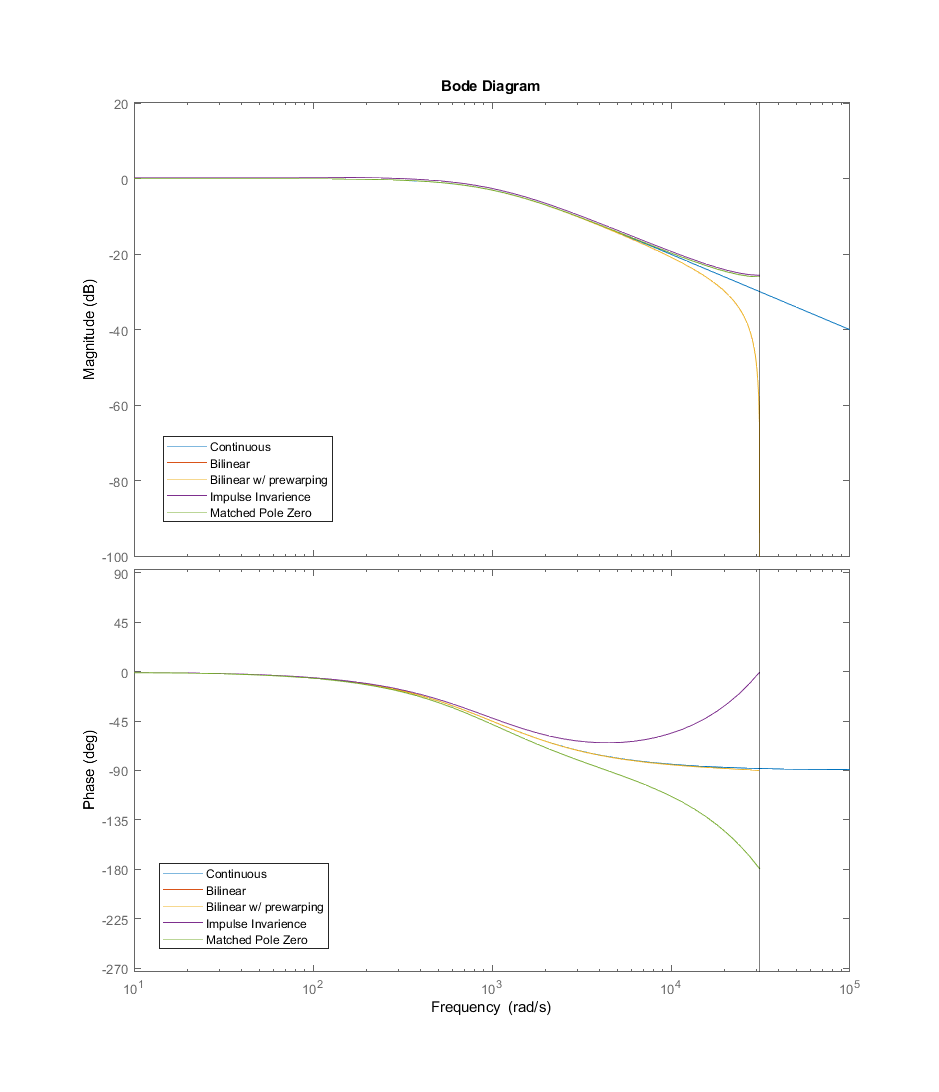
\includegraphics[height=0.3\textwidth]{fig/3_bode.png}
    \end{center}
\end{enumerate}

\section*{Section B - Summative Questions}
\begin{enumerate}
    \item 
    \begin{enumerate}
        \item $$D(s)=e^{st_{d}} = e^{(\sigma+j\omega)t_{d}}$$
        $$e^{j\omega t_d} = cos(\omega t_d) + jsin(\omega t_d)$$
        $$\omega t_d = -\frac{\pi}{2},\; \omega = -\frac{\pi}{2t_d}$$
        \item $$\omega = 1000 rad/s, \; \phi=15^{\circ} = \frac{\pi}{12}$$
        $$t_d = \frac{\pi}{1200}$$
        \item 
            \begin{center}
                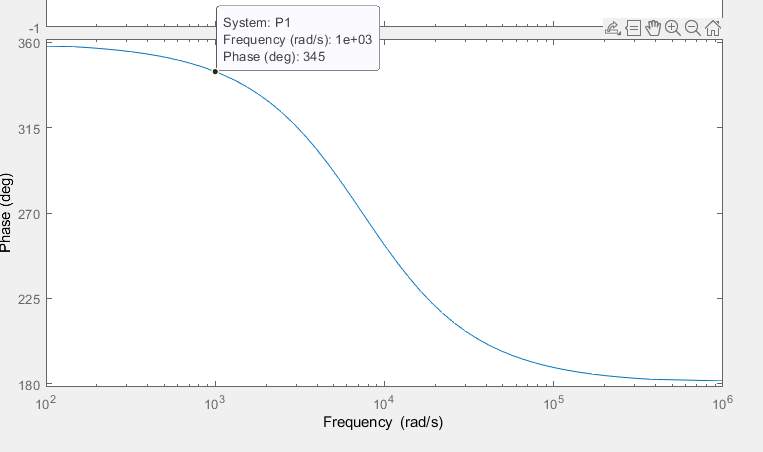
\includegraphics[width=0.3\textwidth]{fig/b1c_270u.png}
                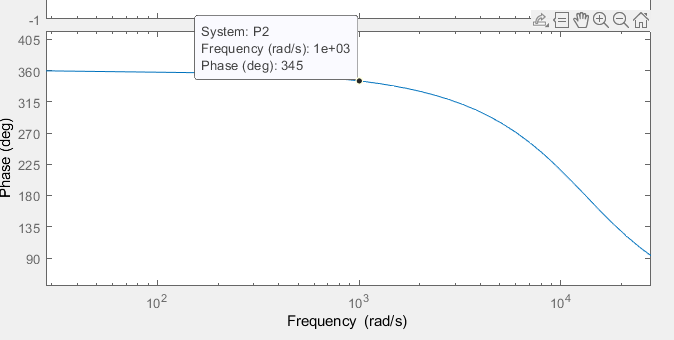
\includegraphics[width=0.3\textwidth]{fig/b1c_2_261u.png}
            \end{center}
    \end{enumerate}
    \item
    $$sampler = \frac{1-e^{st_s}}{s}$$
    $$pade: e^{st_s} \approx \frac{1-s\frac{t_2}{2}}{1+s\frac{t_s}{2}}$$
    $$substitute \rightarrow sampler \approx \frac{2}{s + \frac{s}{t_s}}$$
    \begin{center}
        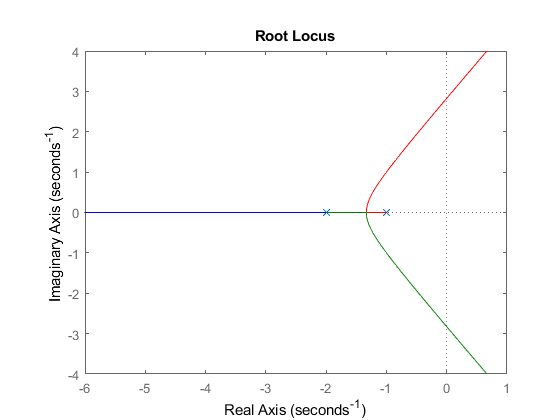
\includegraphics[width=0.25\textwidth]{fig/b2_ts_1_rloc.png}
        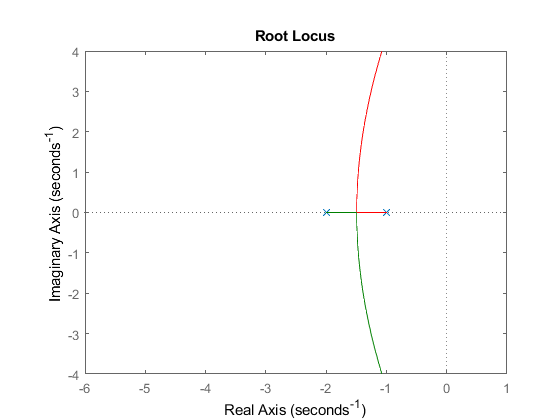
\includegraphics[width=0.25\textwidth]{fig/b2_ts_0.1_rloc.png}
        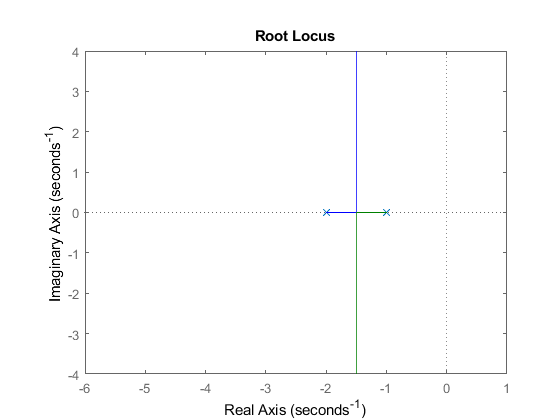
\includegraphics[width=0.25\textwidth]{fig/b2_cont_rloc.png}
    \end{center}
    Sampler effectively inserts a left and pole at 2 / sampling time. Therefore as the sampling speed increases, the inserted pole becomes less and less dominant, the gain margin increases and the system more accurately represents the unsampled system.

    Unity gain frequency is $3.55 rad/s = 0.565Hz$, new sampling: $f = 5.56Hz, t_s = 0.177$
    \begin{center}
        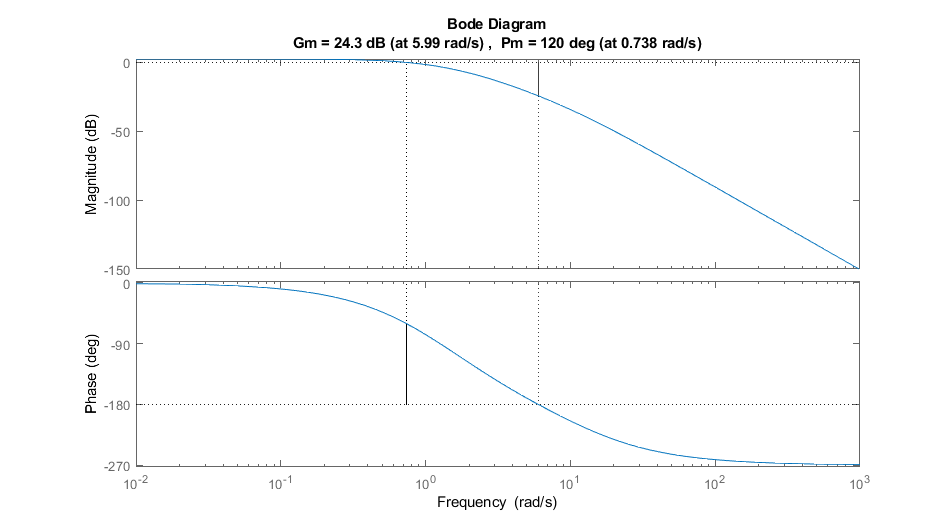
\includegraphics[width=0.3\textwidth]{fig/b2GM.png}
    \end{center}
    \item 
    Corner frequency at 2 decades before sampling frequency to attenuate Nyquist frequency signal by -40dB. 
    $$fs = 1.81Mhz, fc = fs/20$$
    \begin{center}
        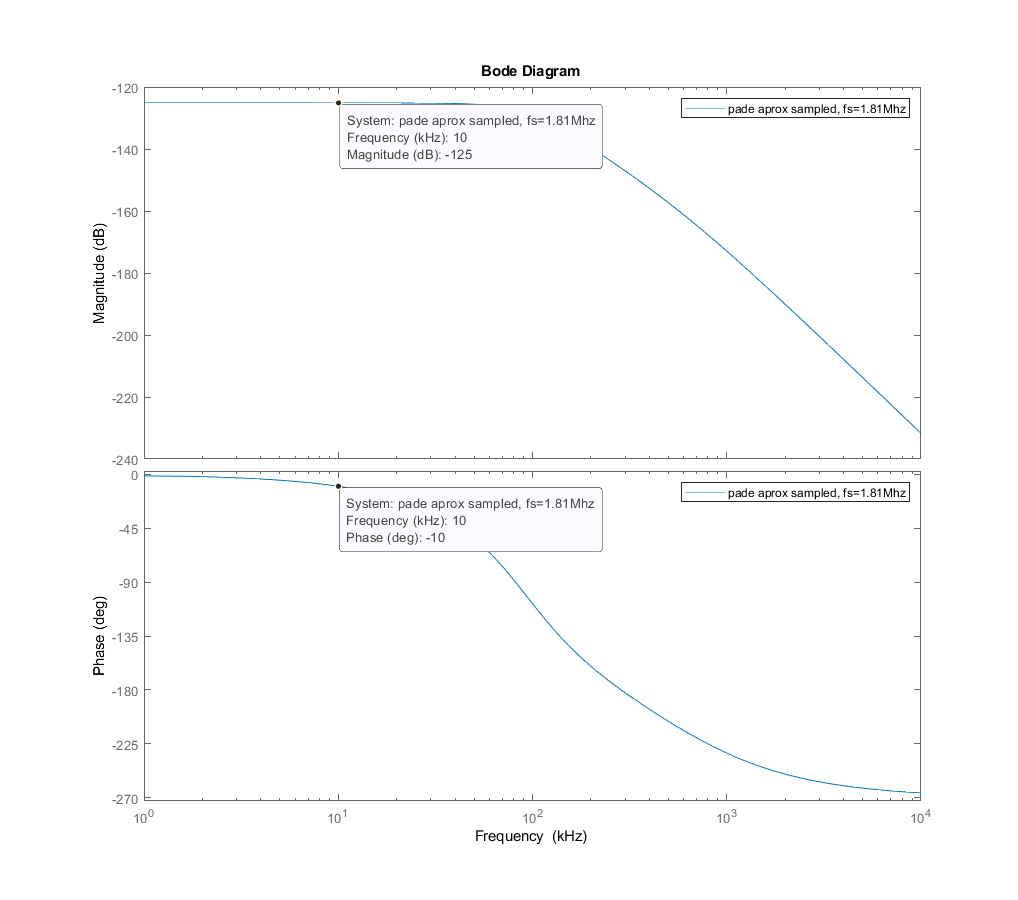
\includegraphics[width=0.3\textwidth]{fig/b3.png}
    \end{center}
\end{enumerate}
\end{preview}
\end{document}